
\section{Background}

\aleksandar{Some short introducing text to this section... this makes segmentation harder, in order to properly assess the sample...}

\subsection{The physical samples}

The physical samples are prepared for SR$\mu$CT scanning by cutting out a portion of a larger
12mm cylindrical sample. \aleksandar{Better to give a brief chronological tour of how the sample has been handled? Time scale also matters to mention in regards to growth.} The cut samples are 6.5mm cubes \aleksandar{more accurate measures?}. This contains the titanium dental implant (Astra Tech OsseoSpeed, ST Molndal, Sweden), which is 3.5mm in diameter and 8mm long. Along its length the lower 5.5mm has larger threads and is attached to recipient bone. The upper 2.5mm has smaller threads and is where newly formed bone is to be assessed. Sorrounding the bone and implant contact-region are cavities containing resin, air, blood vessels and other fibrous tissue. This is shown in figure \ref{fig:3viewsample} \aleksandar{It could perhaps be manually annotated (meaning we can indicate roughly what regions correspond to: resin, air, implant, bone)?}.

\begin{figure}
\centering
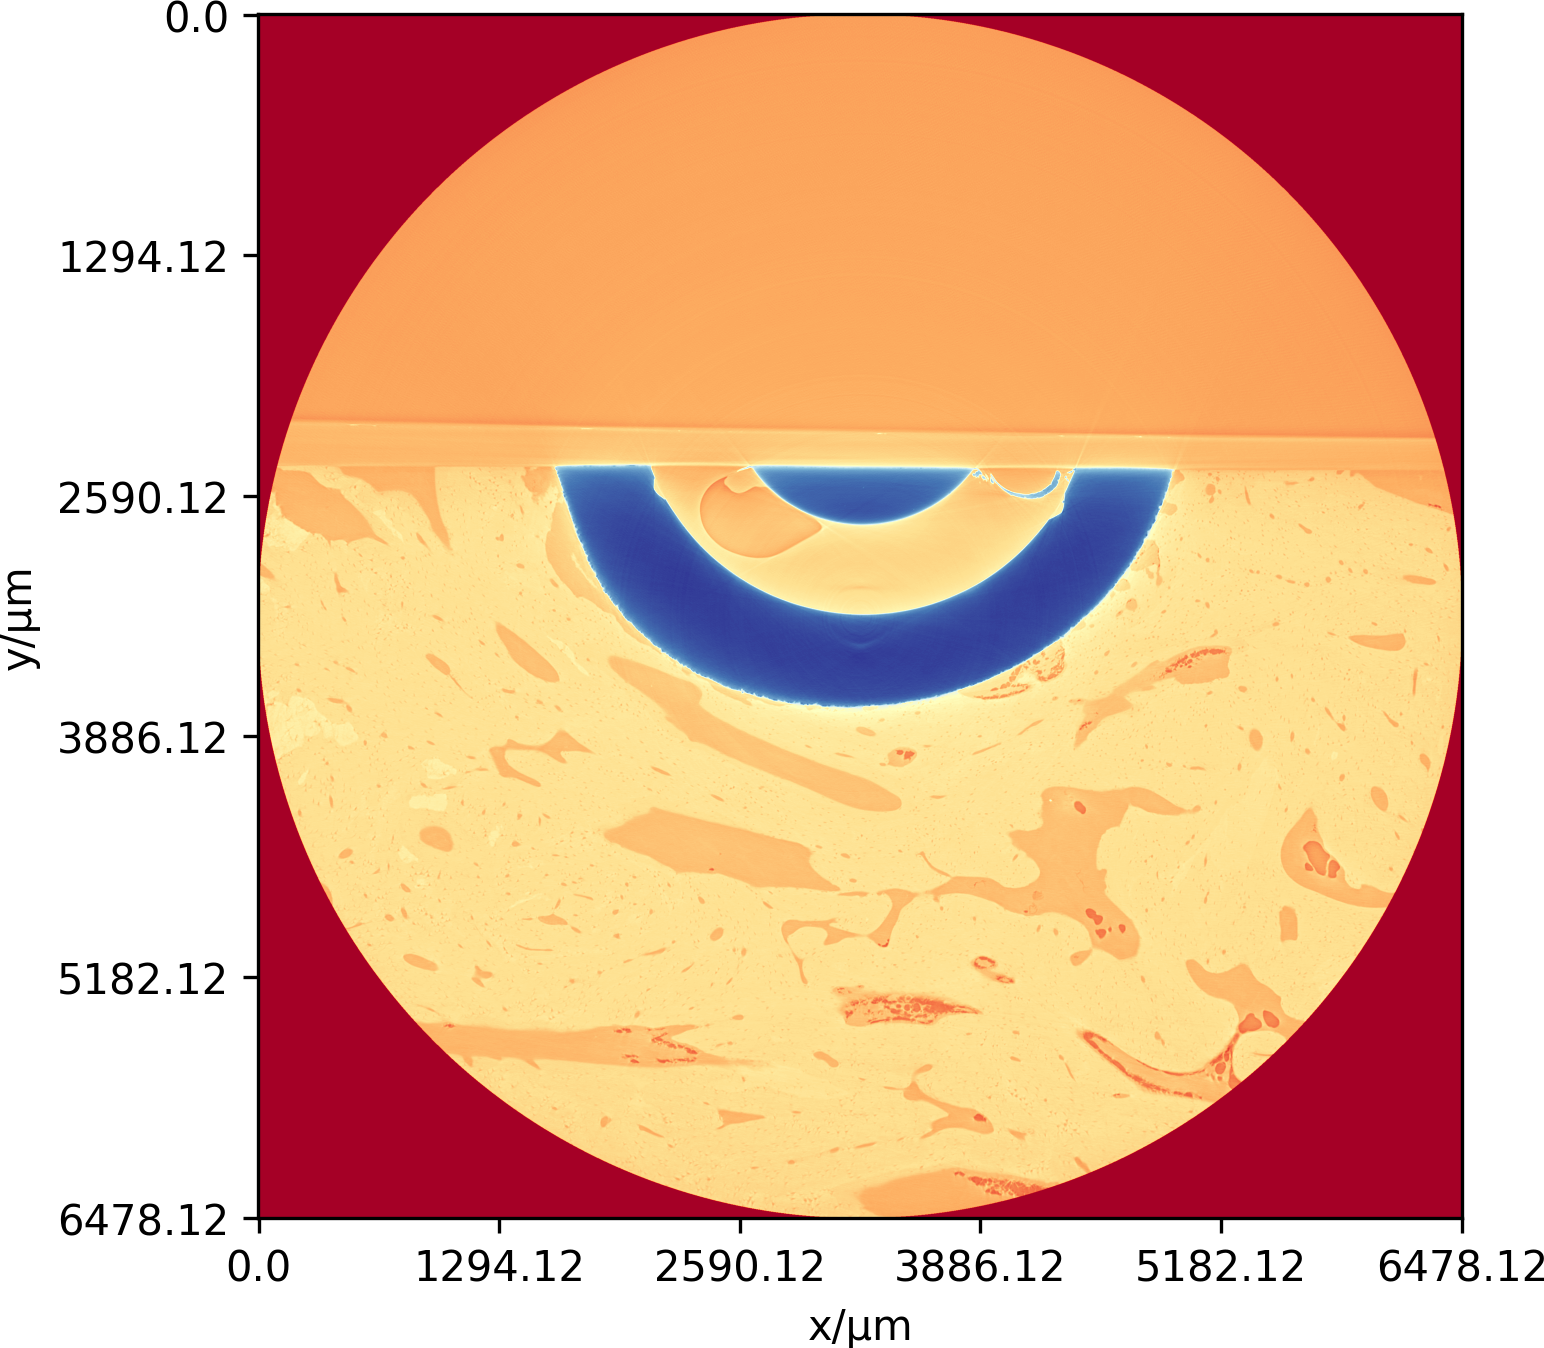
\includegraphics[width=\columnwidth]{figures/770c_pag-full-xy-1x.png}
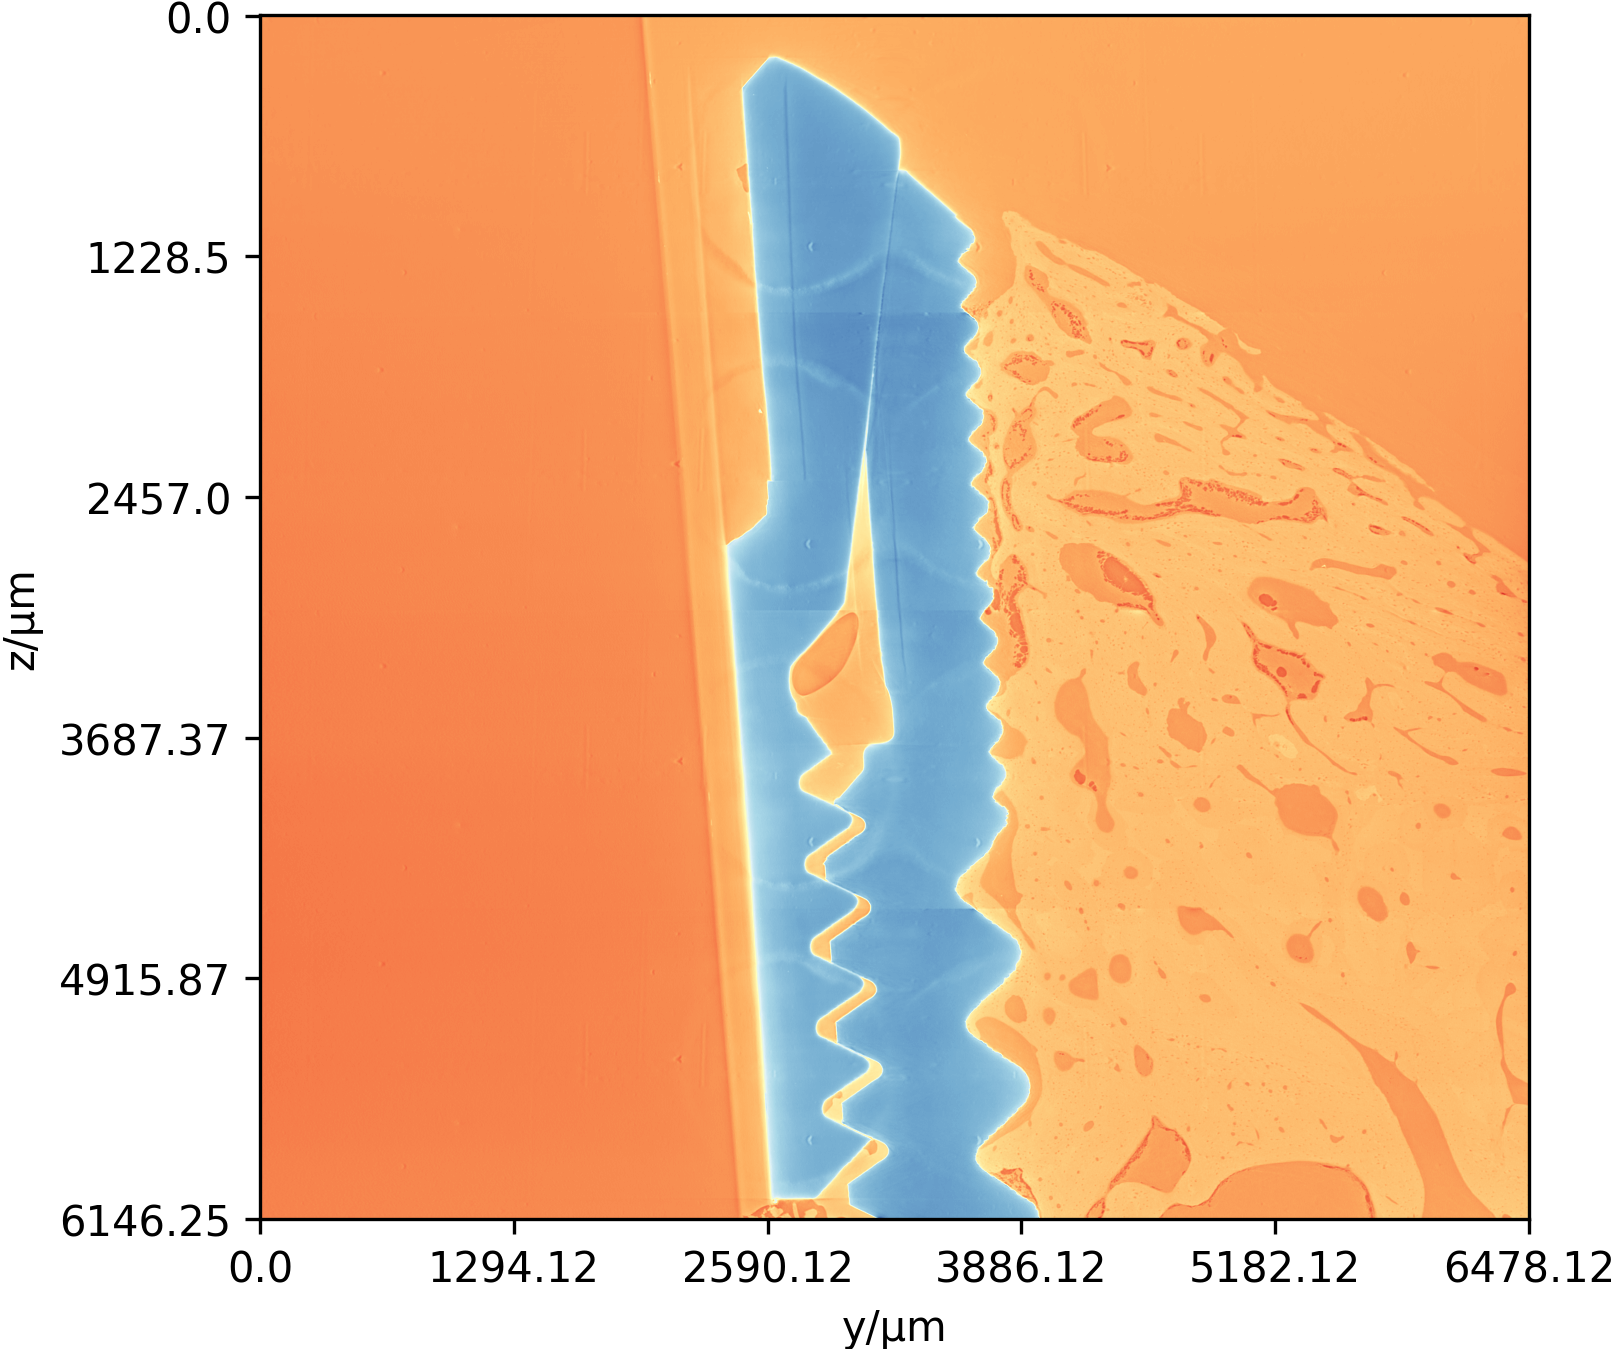
\includegraphics[width=\columnwidth]{figures/770c_pag-full-yz-1x.png}
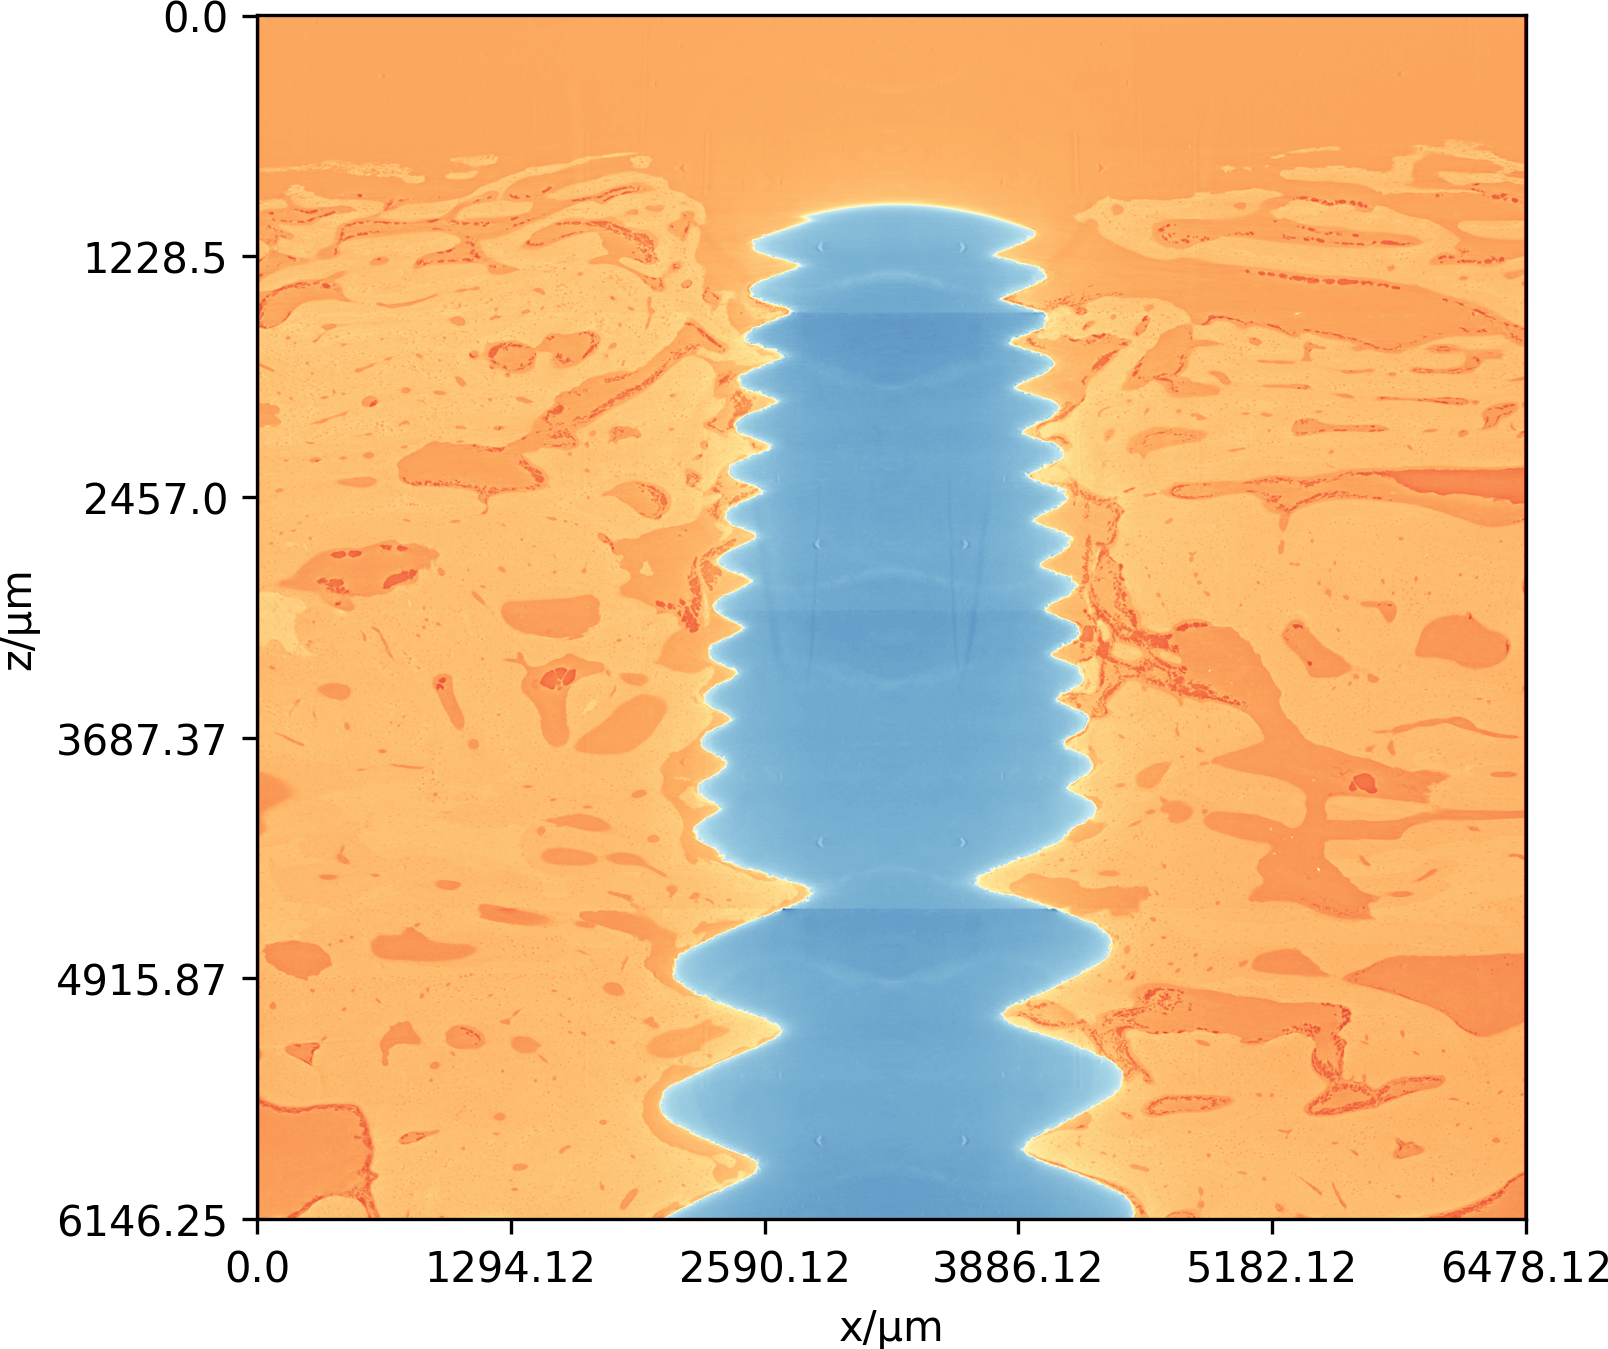
\includegraphics[width=\columnwidth]{figures/770c_pag-full-xz-1x.png}
\caption{Full sample seen from XY, YZ, XZ planes respectively. A voxel has size of 1.875$\mu$m.}
\label{fig:3viewsample}
\end{figure}

Each material has a different density and thus absorption. The titanium implant has higher absorption than bone.
Bone material then has higher absorption than its sorrounding tissue, vessels, air and resin.

\subsection{Data acquisition}

It can be difficult to study and evaluate the bone structure and blood network without destroying or
manipulating the sample. X-ray computed tomography is a widely used tool for non-intrusive medical
imaging. By exposing a subject to X-rays, we can map the linear attentuation coffecient of the passing
rays. Each ray is attenuated relatively to the density and composition of the material it passes. By
rotating either the scanner or the sample we can get a full 3D image representation of the inner
structure of the sample. Each volumetric pixel (voxel) then represents the X-ray attenuation at its spatial position. We can therefore reliably use X-rays to internally characterise samples in a non-intrusive and non-destructive manner.
Regular CT-scans can provide spatial resolutions on the order of millimetre scale.\aleksandar{ref} The more modern micro computed tomography ($\mu$CT) can provide much higher spatial resolution on the micrometre scale.\aleksandar{ref} Both setups utilize poly-energetic beams, which can cause artifacts around high density regions. This effect is called beam-hardening\aleksandar{ref}, and occurs when rays with lower energy are attenuated more frequently. This offsets the local contrast, by overestimating the attenuation, leaving lighter spots on the image. Many other types of artifacts will also occur in these common scanners, but most is taken into account by calibration using phantoms and pre-hardening the beam before it reaches the sample. Due to its common usage, much software also exists to correct for noise and smaller imperfections during reconstruction\aleksandar{ref}.

This work focuses on data acquired by Synchrotron Radiation micro-CT (SR$\mu$CT). For this imaging
technique, electrons are accelerated to ultra-relativistic speeds in trajectories directed by strong
magnetic fields. Contrary to both CT and $\mu$CT, this approach requires a large particle accelerator, and is not standard medical or laboratory equipment\aleksandar{ref}. The added complexity means that SR$\mu$CT can offer an even better spatial resolution of up to 0.1 $\mu$m. The resulting beams are high in brilliance and collimation which gives a very clear signal. Its mono-energetic nature also means that images are not subject to artifacts from beam-hardening.

\aleksandar{Can we confirm whether data was acquired at the ESRF and at which beamline? Also which energies were used? All this could be important for reproducibility.}

\aleksandar{More info on scanner here: https://www.esrf.fr/home/UsersAndScience/Experiments/StructMaterials/ID19/microtomography.html where reconstruction software (pyHST) is also mentioned.}

\aleksandar{add ref to ESRF beam line}

\subsection{Image data}

A single image sample contains voxels with of spatial resolution 1.875$\mu$m. The physical size of
a sample is about 6.5mm, which makes the raw dimensions of a single image $(3480,3480,3384)$ pixels.
For computational purposes, this has been cropped to be divisible by $2^5=32$. A full image sample
is further split into 4-6 sub-volumes through the height of the implant. This gives a size of $(3456,3456,810)$ pixels per sub-volume, where the last axis gets stacked for a full volume.

\aleksandar{OBS: 846 i rå størelse, 810 er efter volume-matching.}

\aleksandar{Important to explain a bit about how the samples were cut during acquisition. How were the samples secured in order not to be shifted too much etc.}

\subsubsection*{XY slice unscaled}

\begin{figure*}%[t]
\centering
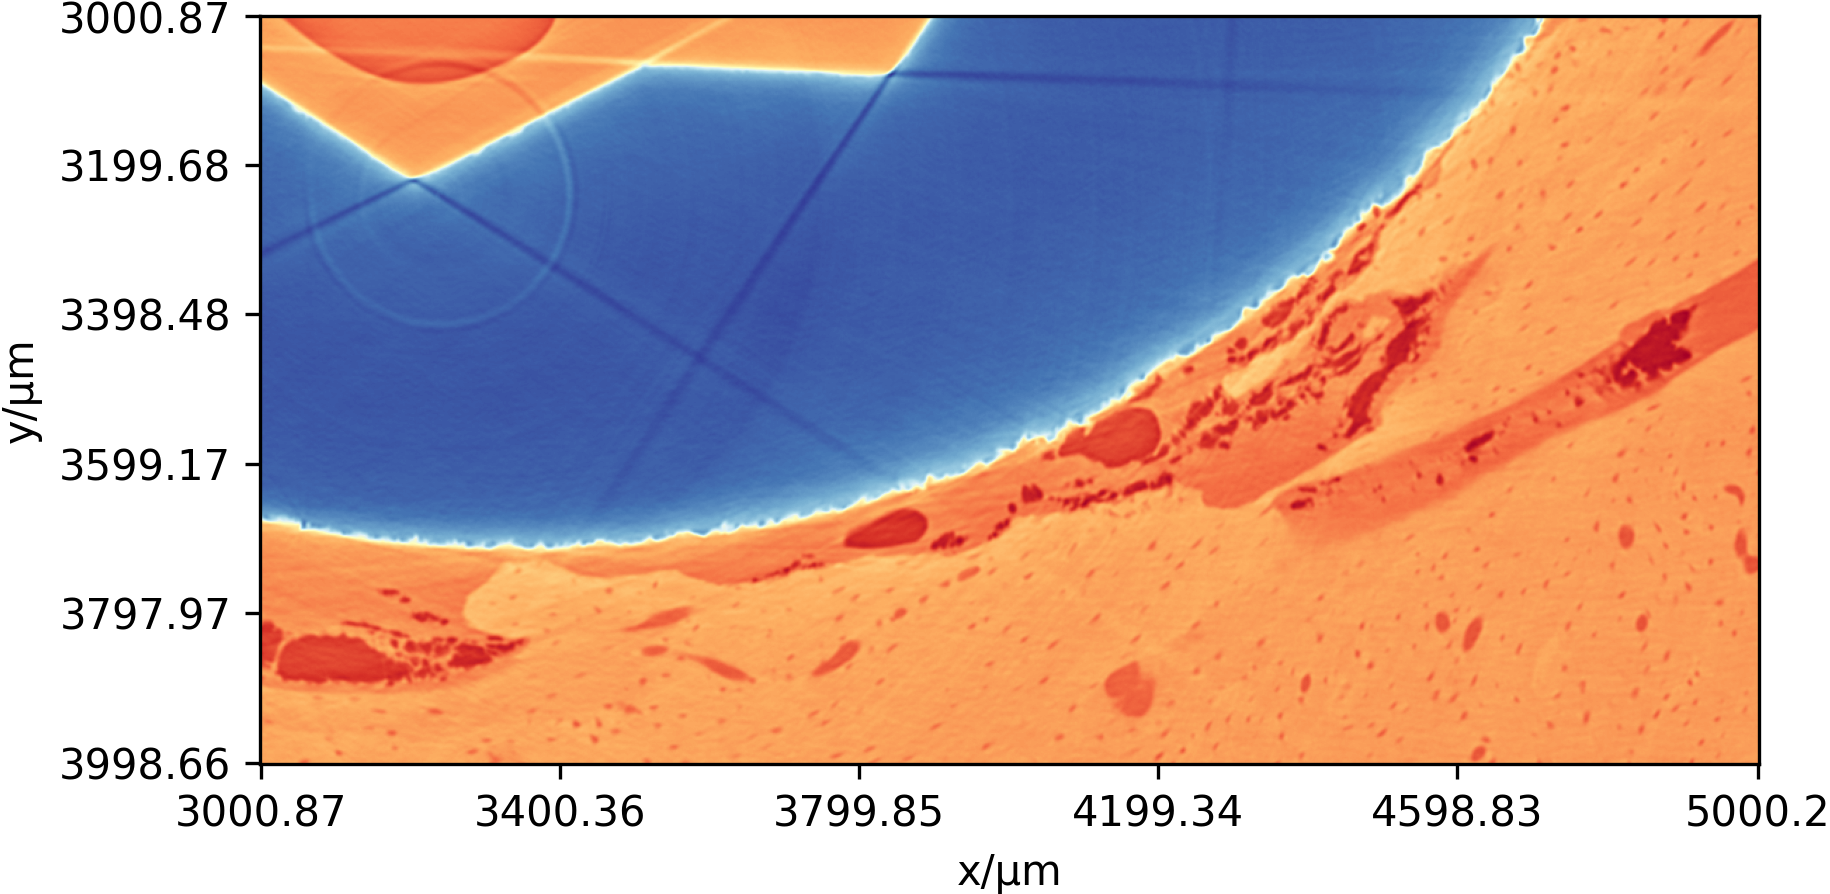
\includegraphics[width=\textwidth]{figures/770c_pag-bic-xy-1x.png}
\caption{Unscaled version of XY-slice.}
\label{fig:xy-slice}
\end{figure*}

\subsubsection*{YZ slice unscaled}

\begin{figure}%[t]
\centering
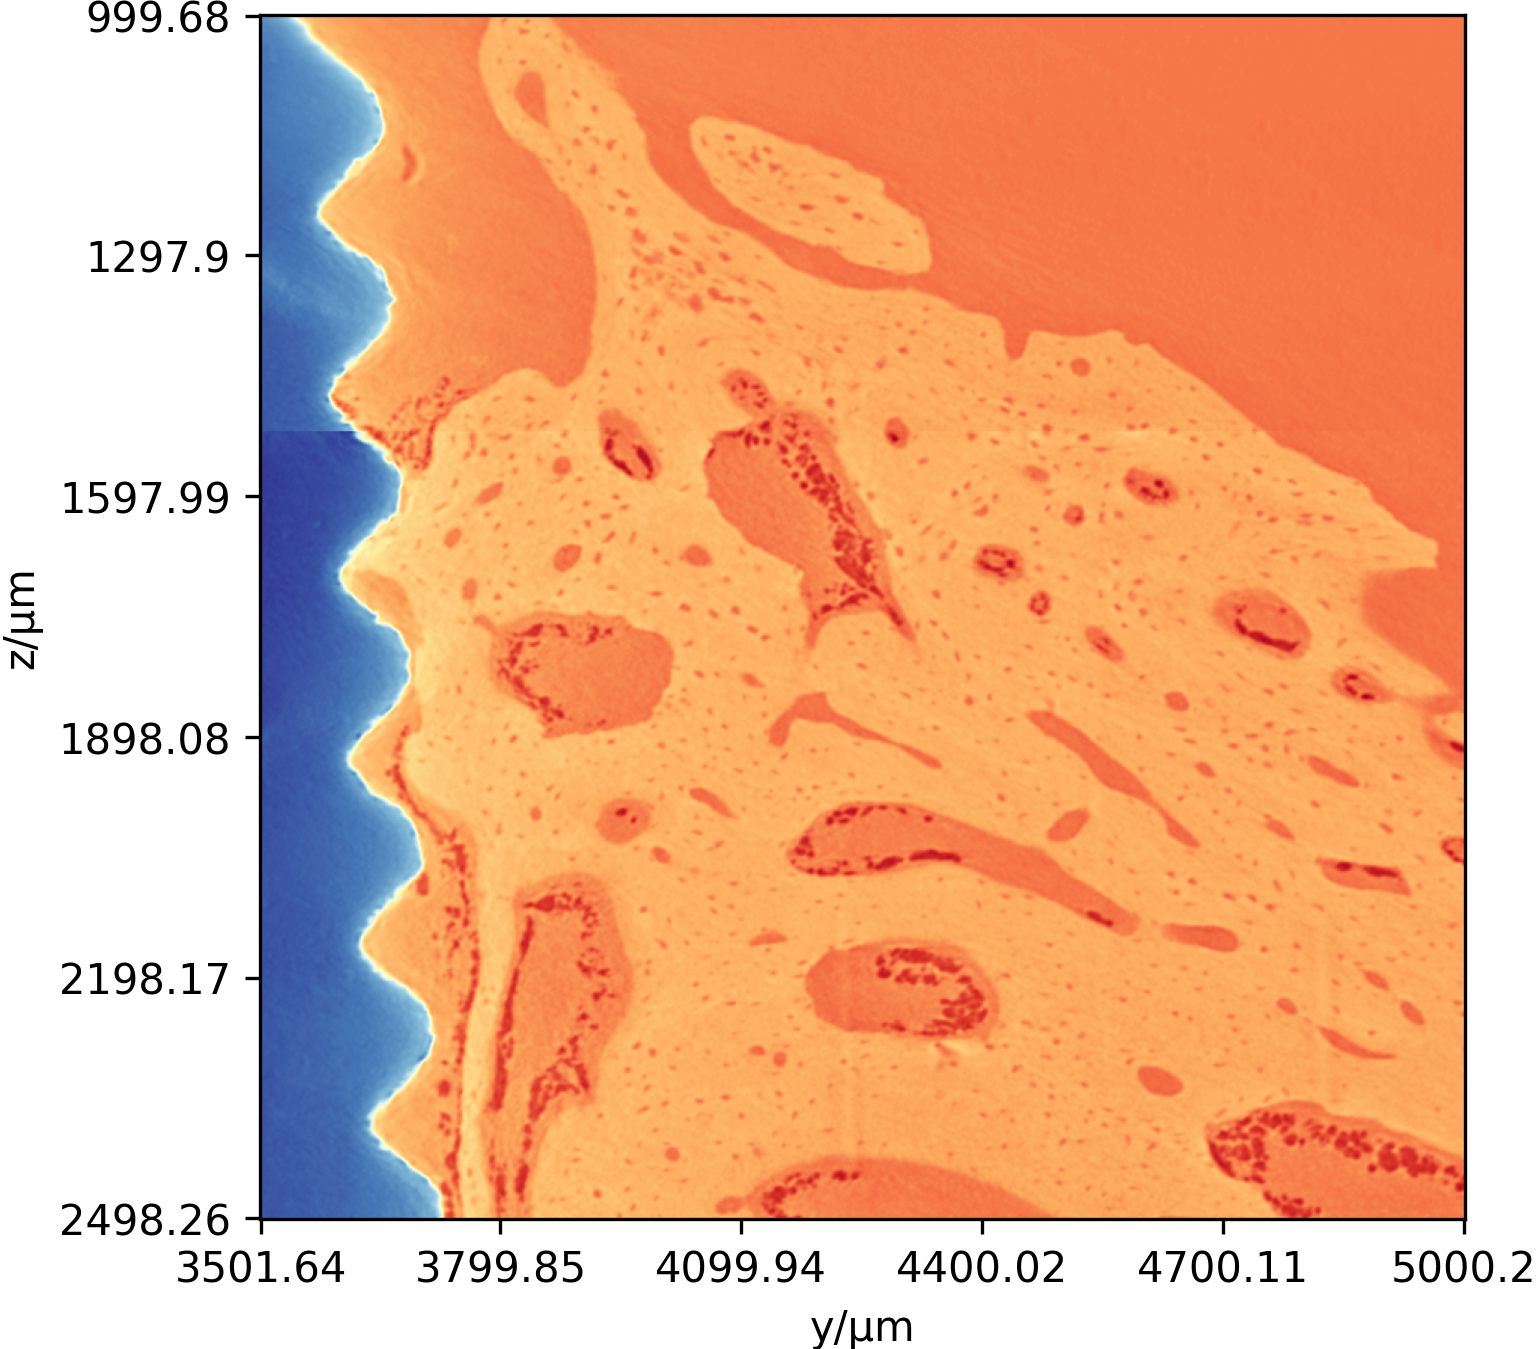
\includegraphics[width=\columnwidth]{figures/770c_pag-bic-yz-1x.png}
\caption{Unscaled version of YZ slice.}
\label{fig:yz-slice}
\end{figure}

\subsection{Physical effects, noise and artifacts}

Noise in tomography is unavoidable, and it makes segmentation harder. Matarials may be well separated from certain angles in the 3d-reconstructed image, but overlap from others. Some noise like that corrected by flat-field correction is very uniformly distributed across images. Some noise is however very spatially dependent on its sorrounding regions. Since we know the compositions of the materials being imaged, we can counter some of these effects during segmentation. The noise effects manifest themselves as numerical shifts in voxel-values as a function of their position. This is a direct result of a misrepresented attenuation along the axis the X-rays are passing. 

\subsubsection{Beam hardening}

Despite the practially mono-energetic rays from SR$\mu$CT, the source initially generates a polychromatic spectrum. During monochromatisation this spectrum can still contain corrupted harmonic components \citep{srnoise}. This leads to two distinct effects typically seen from beam-hardening.

It is the result of lower energy photons being removed in larger amounts, thus
shifting the remaining photons to a higher effective average photon energy. The beam is hardened and only x-rays with sufficient energy to penetrate the object are present.

Softer x-rays will get absorbed instead of successfully penetrating the object,
and will not contribute to image formation. High density structures such as the titanium implant break the isotropy, making the projected X-ray mean energy spectrum dependent on incident orientation \citep{srnoise}.

Beam hardening is typically minimized through pre-hardening of the beam using attenuation filters, along with calibration using phantoms and correction software.

\subsubsection{dark and bright streaks}

Streaking artifacts occur at the dense implant region, but also in the transition from bone to softer tissue.
This effect is mostly seen in regions of large heterogeneity. When X-ray beams pass at angles containing multiple dense obstacles, the beam is hardened more. Then for angles with fewer dense obstacles the energy spectrum is preserved better. This produced the dark and bright streaks seen in \cref{xy}

\subsubsection{cupping effect}

A common artefact that is seen when beams pass cylindrical objects. Since beams passing the middle will traverse more material compared to the edges, the beam is hardened more towards the center and intensity becomes lower as a result. This can manifest itself in what errnoeously looks to be dense peripheral regions at the edges.

\subsubsection{Scattering}

Low energy rays contribute mostly with noise from scattering effects. A ray will propagate through a material, get scattered and diffract from its initial trajectory. This gives a misrepresentation of the attenuation along its initial trajectory.
The artefacts seen from scattering are similar in nature to those formed by beam hardening. This is because both effectively reduce the measured attenuation. ... Low energy bla bla
Also leads to cupping artefact

% Rayleigh, 

\subsubsection{Ring artifacts}

Looking at the XY-slice in figure \cref{xy} we see clear concentric ring artifacts emanating from the center of the sample.
Compared to the other artifacts mentioned, this effect is arising from imperfections in the scanner setup. It can be from an uncalibrated or defect detector element. For synchrotron radiation sources it can also occur from shifts and vibrations in the monochromator crystal \cref{ringartifacts}. 


\subsubsection{Projection artifacts}

Strong edges are seen from the sharp corners of the titanium implant. When doing back projection, this symmetrybreaking is seen as smeared lines across the sample.

\subsubsection{MISC}

\aleksandar{Forklare hvorfor vi ser mørke områder, særligt at det mørke lægger sig omkring implantatet,
men at det så aftager mod knoglen, for så at blive kraftigere og bredere helt ved knoglen..}

\aleksandar{Do we want to include: Undersampling and Poisson noise? Fringes at the edges of the titanium implant due to phase-contrast effects (see srnoise ref), Partial volume artifacts which are dependent on the voxel size and are mentioned briefly by Neldam et al., Refraction noise? When all effects seem to be handled alreayd...}

For SR$\mu$CT a high photon flux allows for very short exposure times \citep{srexptime}.
This can help counter noise from suboptimal counting statistics\citep{srnoise}.
This is for example the case for Poisson noise, which is smaller than.







